%%%%%%%%%%%%%%%%%%%%%%%%%%%%%%%%%%%%%%%%%
% Developer CV
% LaTeX Class
% Version 2.0 (12/10/23)
%
% This class originates from:
% http://www.LaTeXTemplates.com
%
% Authors:
% Omar Roldan
% Based on a template by  Jan Vorisek (jan@vorisek.me)
% Based on a template by Jan Küster (info@jankuester.com)
% Modified for LaTeX Templates by Vel (vel@LaTeXTemplates.com)
%
% License:
% The MIT License (see included LICENSE file)
%
%%%%%%%%%%%%%%%%%%%%%%%%%%%%%%%%%%%%%%%%%

%----------------------------------------------------------------------------------------
%	PACKAGES AND OTHER DOCUMENT CONFIGURATIONS
%----------------------------------------------------------------------------------------

\documentclass[9pt]{developercv} % Default font size, values from 8-12pt are recommended
\usepackage{multicol}
\usepackage{graphicx}
\usepackage{lipsum}
\setlength{\columnsep}{0mm}
%----------------------------------------------------------------------------------------


\begin{document}

%----------------------------------------------------------------------------------------
%	TITLE AND CONTACT INFORMATION
%----------------------------------------------------------------------------------------

\begin{minipage}[t]{0.2\textwidth} 
	\vspace{-\baselineskip} % Required for vertically aligning minipages

		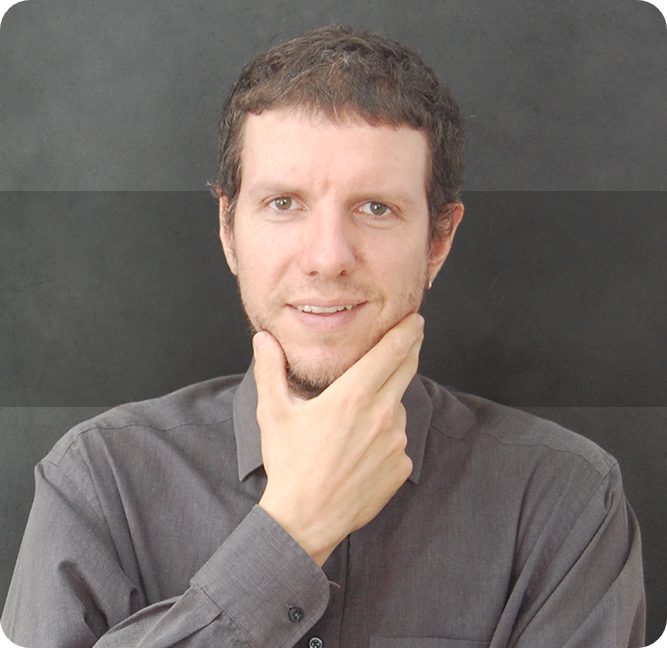
\includegraphics[width=0.7\linewidth]{caio-round.png}
	
\end{minipage}
\begin{minipage}[t]{0.3\textwidth} 
	\vspace{-\baselineskip} % Required for vertically aligning minipages
	
	{ \fontsize{16}{20} \textcolor{black}{\textbf{\MakeUppercase{Caio Laganá \\[1mm]Fernandes}}}} % First name
	
	\vspace{6pt}
	
	{\Large Ph.D Physicist\\[1mm]} % Career or current job title
	Developer
\end{minipage}
\hfill
\begin{minipage}[t]{0.2\textwidth} % 20% of the page width for the first row of icons
	\vspace{-\baselineskip} % Required for vertically aligning minipages
	
	% The first parameter is the FontAwesome icon name, the second is the box size and the third is the text
	\icon{Globe}{11}{\href{http://www.caiolagana.com.br}{caiolagana.com.br}}\\ 
  \icon{Phone}{11}{+55 35 99754 9882}\\
  \icon{MapMarker}{11}{São Paulo, Brazil}\\
	
\end{minipage}
\begin{minipage}[t]{0.27\textwidth} % 27% of the page width for the second row of icons
	\vspace{-\baselineskip} % Required for vertically aligning minipages
	
	\icon{Envelope}{11}{\href{mailto:caiolagana@gmail.com}{caiolagana@gmail.com}}\\	
    \icon{Github}{11}{\href{https://github.com/caiolagana}{github.com/caiolagana}}\\
    \icon{LinkedinSquare}{11}{\href{https://www.linkedin.com/in/caiolagana}{linkedin.com/in/caiolagana}}\\    
    
\end{minipage}

%----------------------------------------------------------------------------------------
%	HEADER
%----------------------------------------------------------------------------------------

\begin{minipage}[t]{0.46\textwidth}
    \cvsect{Summary}
	\vspace{-6pt}

	Possess a Ph.D. in High Energy Nuclear Physics at the European Organization for Nuclear Research (CERN). Awarded the Best Doctorate Thesis Prize by the Brazilian Physical Society in 2020. Experienced in programming languages, software development and data analysis.
\end{minipage}
\hfill % Whitespace between
\begin{minipage}[t]{0.465\textwidth}
    \cvsect{Skills}
    \vspace{-6pt}

	\begin{minipage}[t]{0.35\textwidth}
		\textbf{Portuguese} (native)\vspace{0.5mm}\\
		\textbf{English} (fluent)\vspace{0.5mm}\\
		\textbf{Italian} (fluent)\vspace{0.5mm}\\
		\textbf{French} (functional)\vspace{0.5mm}\\
		\textbf{German} (beginner)
    \end{minipage}
    \hfill
    \begin{minipage}[t]{0.55\textwidth}
	Ability to understand complex systems and work out efficient solutions to intrincate problems
    \end{minipage}
    
\end{minipage}

%----------------------------------------------------------------------------------------
%	PROJECTS
%----------------------------------------------------------------------------------------

\vspace{10 pt}
\cvsect{Projects}
\begin{entrylist}
	\entry
		{C++}
		{Hypernuclei Search at CERN}
		{https://github.com/caiolagana/LnnTTreeCreator}
		{This C++ project was written as part of my Ph.D program. The script was ran over thousands of terabytes of data at CERN's computing infrastructure. It searchs for the $\Lambda nn$ and $\Lambda pn$ hypernuclei in high-energy Pb-Pb collisions at the Large Hadron Collider.}
    \entry
		{Visual C\#, SQL}
		{Hydroelectric Power Plant Simulator}
		{https://github.com/caiolagana/PowerPlantSimulator}
		{Project written in Visual C\# simulating the full scope of a hydroelectric power plant for training operators. A depth-search recursive algorithm is responsible for the electricity power flow, while numerical solution to differential equations emulates the machines.}
    \entry
		{Python, AngularJS}
		{AI Analysis of Legal Documents}
		{https://github.com/e-fluxus/ia}
		{My first project utilizing Artificial Intelligente to extract and analyze data from legal documents. Written in python's FastAPI, integrated with MongoDB and served in a Docker container at AWS. Integrates with an AngularJS front-end.}
		\entry
		{Python}
		{Deep Learning Neural Network for Hand-Written Digits}
		{https://github.com/caiolagana/DeepLearningPython}
		{This is my own implementation of Michael Nielsen's deep learning neural network.}
\end{entrylist}

%----------------------------------------------------------------------------------------
%	FORMAL EDUCATION
%----------------------------------------------------------------------------------------

\vspace{-10 pt}
\cvsect{Formal Education}
\begin{entrylist}
    \entry
		{2013 - 2017}
		{Doctorate in Physics}
		{USP/CERN}
		{University of São Paulo (USP) with one-year exchange program at European Organization for Nuclear Research (CERN). {\it Title:} Evidence for the existence of the $\Lambda nn$ hypernucleus with the ALICE detector}
    \entry
		{2010-2012}
		{Master's in Physics}
		{UNESP}
		{State University of São Paulo (UNESP) {\it Title:} Femtoscopia de colisões próton-próton no detector CMS do Large Hadron Collider}
	\entry
		{2006-2010}
		{Bachelor's in Physics}
		{USP}
		{Scholarship from Conselho Nacional de Desenvolvimento Científico e Tecnológico (CNPq)}
\end{entrylist}

%----------------------------------------------------------------------------------------
%	COMPLEMENTARY EDUCATION
%----------------------------------------------------------------------------------------

\vspace{-10 pt}
\cvsect{Complementary Education}
\begin{entrylist}
    \entry
		{2012}
		{Excellence in Detectors and Instrumentation Technologies}
		{Fermilab}
		{Fermi National Accelerator Laboratory, Illinois (US)}
	\entry
		{2012}
		{Short Term Course in Laboratory Techniques}
		{BNL}
		{Brookhaven National Laboratory, Upton (US)}
	\entry
		{2010}
		{Short Term Course in Data Analysis Tools at CERN}
		{CERN}
		{European Organization for Nuclear Research, Meyrin (Switzerland)}
\end{entrylist}

%----------------------------------------------------------------------------------------
%	EXPERIENCE
%----------------------------------------------------------------------------------------

\vspace{-10 pt}
\cvsect{Experience}
\begin{entrylist}
	\entry
        {2014}
		{Assistant Professor}
		{IFUSP}
		{\vspace{-10pt}
        \begin{itemize}[noitemsep,topsep=0pt,parsep=0pt,partopsep=0pt, leftmargin=-1pt]
            \item Working hours (weekly): 6h
            \item Course: Laboratório de Física Moderna
        \end{itemize}
		}
	\entry
        {2017 - 2019}
		{Visual C\# Developer}
		{AQS Tecnologia}
		{\vspace{-10pt}
        \begin{itemize}[noitemsep,topsep=0pt,parsep=0pt,partopsep=0pt, leftmargin=-1pt]
            \item Working hours (weekly): 40h
        \end{itemize}
		}
	\entry
        {2019}
		{Scientific Journal Referee}
		{USP}
		{\vspace{-10pt}
        \begin{itemize}[noitemsep,topsep=0pt,parsep=0pt,partopsep=0pt, leftmargin=-1pt]
            \item Physical Science International Journal
        \end{itemize}
		}
	\entry
        {2020}
		{Scientific Journal Referee}
		{USP}
		{\vspace{-10pt}
        \begin{itemize}[noitemsep,topsep=0pt,parsep=0pt,partopsep=0pt, leftmargin=-1pt]
            \item Caderno Brasileiro de Ensino de Física
        \end{itemize}
		}
	\entry
        {2021}
		{Assistant Professor}
		{POLI-USP}
		{\vspace{-10pt}
        \begin{itemize}[noitemsep,topsep=0pt,parsep=0pt,partopsep=0pt, leftmargin=-1pt]
            \item Working hours (weekly): 6h
            \item Course: Física III
        \end{itemize}
		}
	\entry
        {2022 - Current}
		{Python Developer}
		{E-FLUXUS}
		{\vspace{-10pt}
        \begin{itemize}[noitemsep,topsep=0pt,parsep=0pt,partopsep=0pt, leftmargin=-1pt]
            \item Working hours (weekly): 40h
        \end{itemize}
		}
\end{entrylist}

%----------------------------------------------------------------------------------------
%	AWARDS
%----------------------------------------------------------------------------------------

\vspace{-10 pt}
\cvsect{Awards}
\begin{entrylist}
    \entry
		{2013}
		{Best Panel Prize of the XXXVI Reunião de Trabalho sobre Física Nuclear no Brasil}
		{SBF}
		{Master's Degree}
	\entry
		{2020}
		{Best Doctorate Thesis Prize by the Brazilian Physical Society}
		{SBF}
		{Doctorate Degree}
\end{entrylist}

%----------------------------------------------------------------------------------------
%	PUBLICATIONS
%----------------------------------------------------------------------------------------

\vspace{-10 pt}
\cvsect{Publications}
\begin{entrylist}
	\entry
        {2018}
		{Production of deuterons, tritons, $^3$He nuclei, and their antinuclei in $pp$ collisions}
		{}
		{Phyis. Rev. C {\bf 97} p.024615}
	\entry
        {2018}
		{Production of $^4$He and $^4$\overline{\mbox{He}}$ in Pb-Pb collisions at $\sqrt{s_{NN}}=2.76$ TeV at the LHC}
		{}
		{Nucl. Phys. A {\bf 971} p.1-20}
	\entry
        {2017}
		{Measurement of the mass difference between top quark and antiquark in $pp$ collisions}
		{}
		{Phys. Lett. B {\bf 770} p.50-71}
	\entry
        {2016}
		{$^3_\Lambda$H and $^3_\overline{\Lambda}$$\overline{\mbox{H}}$ production in Pb-Pb collisions at $\sqrt{s_{NN}}=2.76$ TeV}
		{}
		{Phys. Lett. B {\bf 754} p.360-372}
	\entry
        {2015}
		{Precision measurement of the mass difference between light nuclei and anti-nuclei}
		{}
		{Nature Physics {\bf 11} p.811-814}
	\entry
        {2015}
		{Two-pion femtoscopy in p-Pb collisions at $\sqrt{s_{NN}}=5.02$ TeV}
		{}
		{Phys. Rev. C {\bf 91} p.034906}
	\entry
		{2014}
		{Spectroscopic version of the Aharonov-Bohm effect}
		{}
		{C. Laganá Fernandes, \href{https://arxiv.org/abs/1403.6700}{arXiv:1403.6700}}
	\entry
        {2013}
		{Decaimentos nucleares em uma câmara de nuvens}
		{}
		{C. Laganá Fernandes, Revista Brasileira de Ensino de Física {\bf 35} p.3314}
	\entry
        {2011}
		{Estudo de raios cósmicos utilizando uma câmara de nuvens de baixo custo}
		{}
		{C. Laganá Fernandes, Revista Brasileira de Ensino de Física {\bf 33} p.3302}
	\end{entrylist}



\end{document}